\documentclass[18pt]{beamer}
\usetheme{Madrid}

\usepackage{graphics}


\newcommand{\centeredlargetext}[3]{
{
\setbeamertemplate{navigation symbols}{}
\setbeamercolor{background canvas}{bg={#1}}
\color{#2}
\begin{frame}[plain]
\fontsize{36pt}{36pt}\selectfont
\center
\begin{center}
{#3}
\end{center}
\end{frame}
}}

\newcommand{\centeredhugetext}[3]{
{
\setbeamertemplate{navigation symbols}{}
\setbeamercolor{background canvas}{bg={#1}}
\fontsize{72pt}{72pt}\selectfont
\color{#2}
\begin{frame}[plain]
\center
\begin{center}
{#3}
\end{center}
\end{frame}
}}


\begin{document}

\title[ITKv4]{ITKv4 - The Next Generation}
\subtitle[ITKv4]{What is new in ITKv4}
\institute[Insight Software Consortium]{Insight Software Consortium}
\date[June 2011]{June 2011}

\begin{frame}
\titlepage
\end{frame}


{
\setbeamertemplate{navigation symbols}{}
\begin{frame}[plain]
\center
\begin{center}
This presentation is copyrighted by\\
The \textbf{Insight Software Consortium}\\
\bigskip
distributed under the\\
\textbf{Creative Commons by Attribution License 3.0}\\
\url{http://creativecommons.org/licenses/by/3.0}\\
\end{center}
\end{frame}
}


\begin{frame}
  \tableofcontents
\end{frame}


\centeredlargetext{white}{black}{
ITKv4
}


\centeredlargetext{white}{black}{
10 Years Old
}

\centeredlargetext{white}{black}{
\$ 5 Million
}

\centeredlargetext{white}{black}{
ARRA Funds
}

\centeredlargetext{white}{black}{
1.5 Years
}

\centeredlargetext{white}{black}{
Next 10 Years
}

\centeredlargetext{black}{white}{
Apache 2.0 License
}

\centeredlargetext{black}{white}{
Patented Directory\\
Removed
}


\centeredlargetext{white}{black}{
New Software Process
}

\begin{frame}
\frametitle{Software Process}
\Huge
\begin{itemize}
\item Git
\pause
\item Gerrit
\pause
\item cdash@home
\pause
\item Improved Testing Data
\end{itemize}
\end{frame}


\centeredlargetext{black}{white}{
Modern C++
}


\begin{frame}
\frametitle{Deprecated Compilers}
\Huge
\begin{itemize}
\item Visual Studio 6.0, 7.0
\pause
\item Borland 5.5
\pause
\item Sun CC $<$ 5.9
\pause
\item SGI CC
\pause
\item MWORKS
\pause
\item Cygwin
\pause
\item GCC $<$ 3.4
\end{itemize}
\end{frame}



\centeredlargetext{black}{white}{
64 Bits
}


\begin{frame}
\frametitle{64 Bits}
\Huge
\begin{itemize}
\item Since 2008
\pause
\item In Windows 64bits:\\unsigned long is 32bits
\pause
\item Use typedef !
\pause
\item ITK\_USE\_64BITS\_IDS
\end{itemize}
\end{frame}




\centeredlargetext{white}{black}{
Modularization
}

\begin{frame}
\frametitle{Modularization}
\Huge
\begin{itemize}
\item 98 Modules
\pause
\item Groups
\pause
\item External Modules
\end{itemize}
\end{frame}


{
\setbeamertemplate{navigation symbols}{}
\setbeamertemplate{background canvas}{
  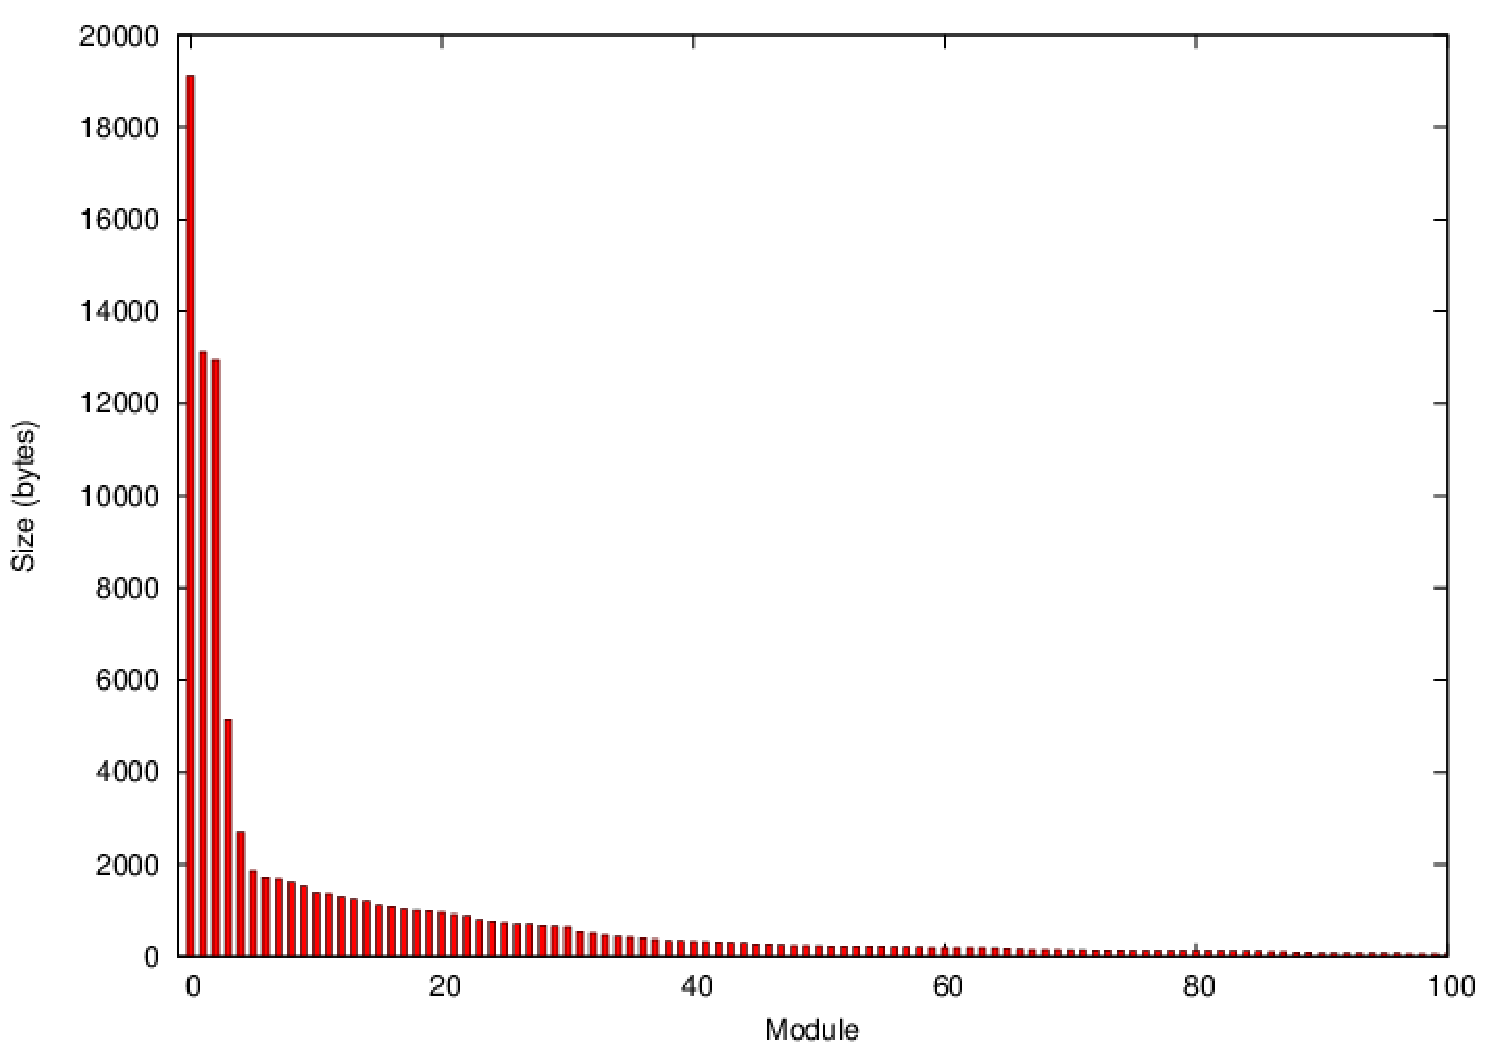
\includegraphics[width=\paperwidth,height=\paperheight]{moduleSizePlot.pdf}
}
\begin{frame}[plain]
\end{frame}
}


{
\setbeamertemplate{navigation symbols}{}
\setbeamertemplate{background canvas}{
  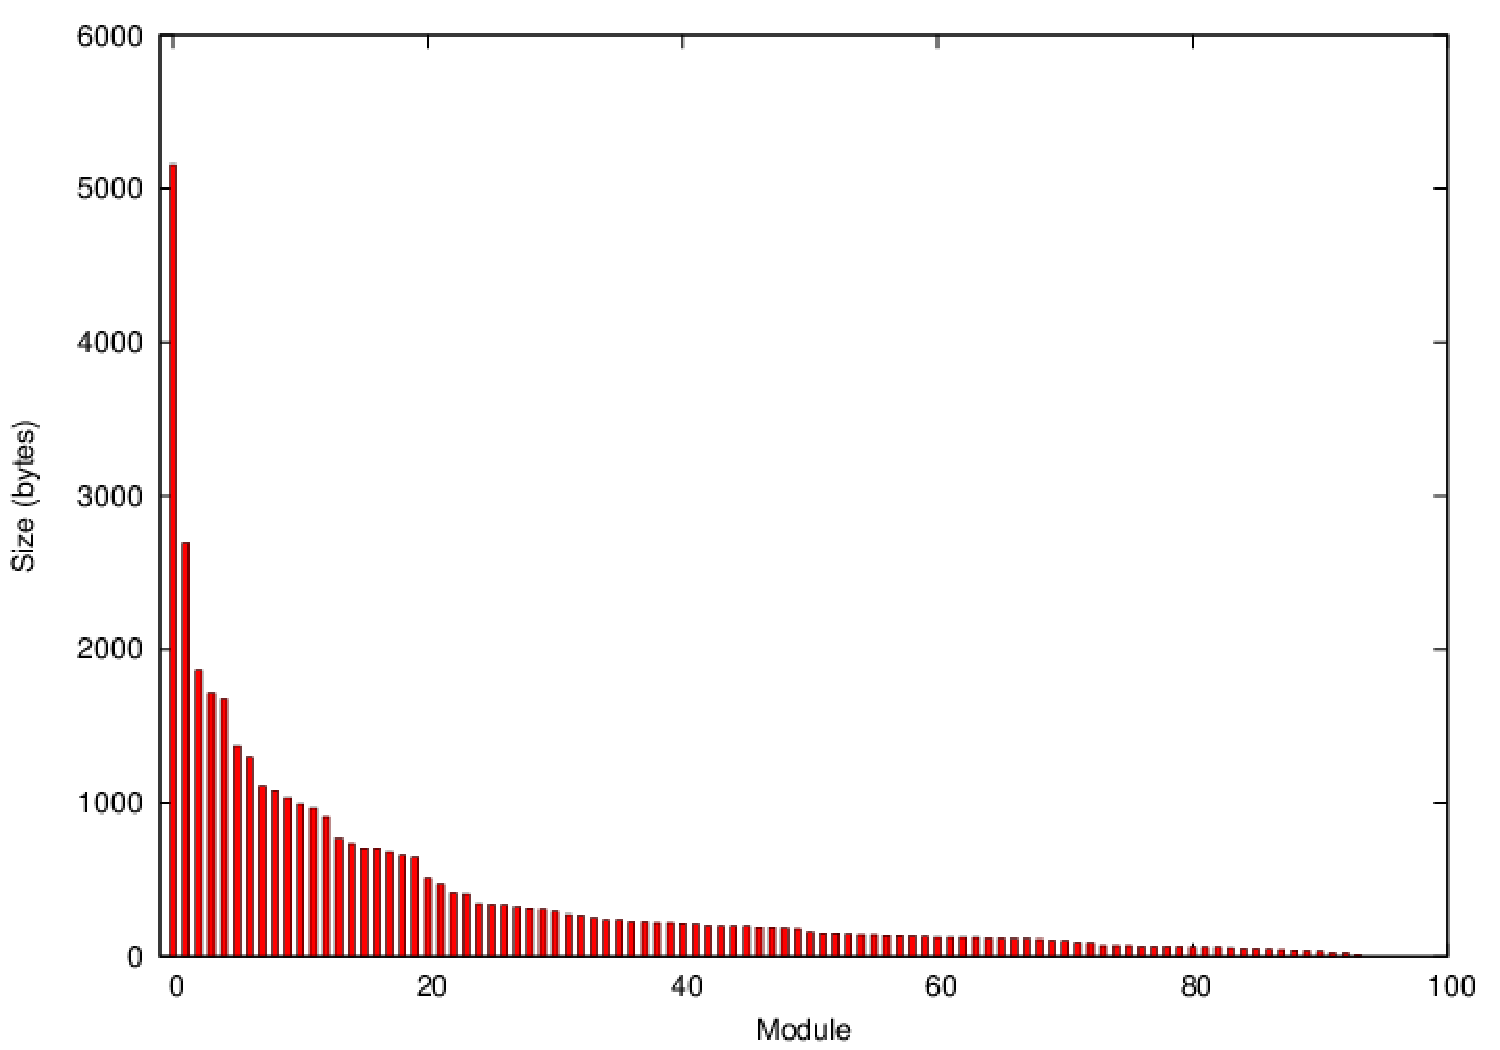
\includegraphics[width=\paperwidth,height=\paperheight]{moduleSizePlotNoThirdParty.pdf}
}
\begin{frame}[plain]
\end{frame}
}


\centeredlargetext{white}{black}{
Statistics Framework
}


\centeredlargetext{black}{white}{
DICOM
}


\begin{frame}
\frametitle{DICOM}
\Huge
\begin{itemize}
\item GDCM 2.0
\pause
\item Query / Retrieve
\pause
\item RT Struct
\end{itemize}
\end{frame}




\centeredlargetext{white}{black}{
FEM Refactoring
}

\begin{frame}
\frametitle{FEM Refactoring}
\Huge
\begin{itemize}
\item Code Clean up
\pause
\item Removed subversive pointers
\pause
\item FEM IO
\end{itemize}
\end{frame}


\centeredlargetext{white}{black}{
Level Sets Refactoring
}

\begin{frame}
\frametitle{Level Sets Refactoring}
\Huge
\begin{itemize}
\item Generalization for Images and Meshes
\pause
\item Modular Terms
\end{itemize}
\end{frame}


\centeredlargetext{white}{black}{
Image Registration Refactoring
}

\begin{frame}
\frametitle{Image Registration Refactoring}
\Huge
\begin{itemize}
\item Composite Transform
\pause
\item Symmetric Registration
\pause
\item Transforms IO
\end{itemize}
\end{frame}


\centeredlargetext{black}{white}{
Registration\\
Parameter Tunning
}


\centeredlargetext{white}{black}{
GPU
}


\begin{frame}
\frametitle{GPU}
\Huge
\begin{itemize}
\item GPU Module
\pause
\item GPU Image
\pause
\item GPU ImageToImageFilter
\pause
\item Factories
\end{itemize}
\end{frame}


\centeredlargetext{white}{black}{
SimpleITK
}


\begin{frame}
\frametitle{SimpleITK}
\Huge
\begin{itemize}
\item Hiding Templates
\pause
\item Smarter IO
\pause
\item Procedural Programming
\pause
\item Easier Wrapping
\pause
\item Binary Distribution
\end{itemize}
\end{frame}


\centeredlargetext{white}{black}{
New Fields
}


\begin{frame}
\frametitle{New Fields}
\Huge
\begin{itemize}
\item Microscopy
\pause
\item Video
\pause
\item Remote Sensing
\end{itemize}
\end{frame}


\centeredlargetext{white}{black}{
Video Bridge
}


\begin{frame}
\frametitle{Video Bridge}
\Huge
\begin{itemize}
\item OpenCV
\pause
\item VXL
\pause
\item Video Filters
\end{itemize}
\end{frame}


\centeredlargetext{black}{white}{
Video Grabber
}


\begin{frame}
\frametitle{Video Grabber}
\Huge
\begin{itemize}
\item Laparoscopy
\pause
\item Ultrasound
\end{itemize}
\end{frame}


\centeredlargetext{white}{black}{
Microscopy
}


\begin{frame}
\frametitle{Microscopy}
\Huge
\begin{itemize}
\item Deconvolution
\pause
\item Denoising
\pause
\item Color correction
\pause
\item Colocalization
\pause
\item File Formats
\end{itemize}
\end{frame}


\centeredlargetext{black}{white}{
Large Images
}


\begin{frame}
\frametitle{Large Images}
\Huge
\begin{itemize}
\item JPEG 2000
\pause
\item Tiling
\pause
\item HDF5
\pause
\item Multi-Resolution Levels
\end{itemize}
\end{frame}


\centeredlargetext{black}{white}{
Insight Journal
}

\begin{frame}
\frametitle{Insight Journal}
\Huge
\begin{itemize}
\item Git Backend
\pause
\item Virtual Appliances
\pause
\item CDE
\pause
\item Reproducible Research
\end{itemize}
\end{frame}


\centeredlargetext{black}{white}{
Migration Guide
}


\centeredlargetext{black}{white}{
\url{http://ij.itk.org/itkfaq}
}


\centeredlargetext{white}{black}{
Live Long\\
and\\
Prosper !
}


\end{document}
